تاخیرهای زیر را برای بخش‌های مختلف شکل زیر در نظر می‌گیریم:

\setLTR

$\qquad\qquad\quad\qquad\qquad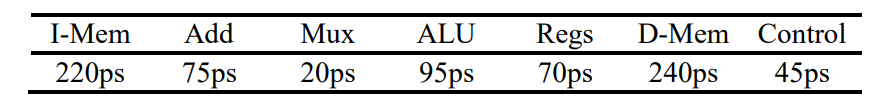
\includegraphics[width=0.5\linewidth]{figs/7.png}$

\setRTL

\setLTR

$\qquad\qquad\qquad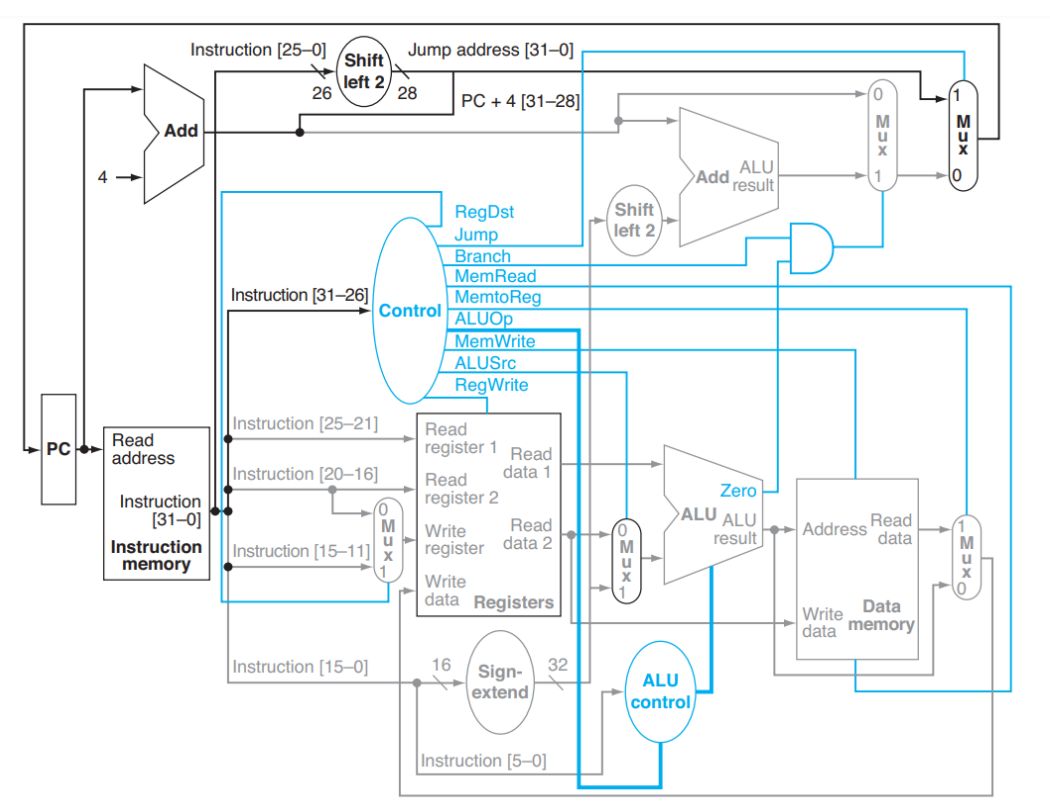
\includegraphics[width=0.7\linewidth]{figs/6.png}$

\setRTL

ابتدا تاخیرهای هر بخش را محاسبه می‌کنیم:

\begin{itemize}
	\item پرش غیر شرطی:
	
	\setLTR
	$\max(IMem,Add) + MUX + Control = 220 + 20  +45=285^{ps}$
	\setRTL
	
	\item پرش شرطی:

\setLTR
$\max(IMem,Add) + \max(Control,Regs) + MUX + \max(ALU,Add) + 2\times MUX \linebreak =
220 + 70 + 20 + 95 + 2\times40= 445^{ps}
$
\setRTL

	\item :Load

\setLTR
$\max(IMem,Add) + \max(Control,Regs) + MUX + ALU + DMem + MUX + Regs \linebreak = 220 + 70 + 20 + 95 + 240 + 20 + 70 = 735^{ps}
$
\setRTL

	\item :Store

\setLTR
$\max(IMem,Add) + \max(Control,Regs) + MUX + ALU + DMem \linebreak = 220 + 70 + 20 + 95 + 240  = 645^{ps}
$
\setRTL

	\item :RType

\setLTR
$\max(IMem,Add) + \max(Control,Regs) + MUX + ALU + MUX + Regs \linebreak = 220 + 70 + 20 + 95 + 20 + 70  = 495^{ps}
$\\ \\
\setRTL
\end{itemize}

\setLTR

$T_1 = \frac{8}{100} \times 285 + \frac{11}{100} \times 445 +\frac{16}{100} \times 735 + \frac{15}{100} \times 645 +\frac{50}{100} \times 515  = 543.6^{ps}$

$T_2 = \frac{8}{100} \times 295 + \frac{11}{100} \times 435 +\frac{16}{100} \times 665 + \frac{15}{100} \times 575 +\frac{50}{100} \times 505  = 516.6^{ps}$ \\ \\



$SpeedUP = \frac{T_1}{T_2} = \frac{543.6}{516.6} \approx 1.05$
\setRTL

پس ما تقریبا 5\% افزایش سرعت داشته‌ایم!